%
% error.tex
%
\section{Chart::ErrorBars}
\name{Chart::ErrorBars}
\file{ErrorBars.pm}
\requires{Chart::Base, GD, Carp, FileHandle}

\begin{Description} 
\class{ErrorBars} is a subclass of \class{Chart::Base}.
The class \class{ErrorBars} creates a point chart with error bars.\\
Chart expects the error values within the data array. 
By use of the \method{add\_dataset()} method the error values are the next two sets after the y values. The first set after the y values has to be a set values for the upper error bars. 
The next set is an array of the down errors.\\
If you want to use the same value for the up and down error, then you have to set the 
'same\_error' option to 'true'. In this case only one set after the y values is interpreted 
as a set of errors.\\
Of course, it's also possible to use the \method{add\_pt()} method in a respective way.
\end{Description}

\parindent 0pt{\large Example:}
\begin{figure}[h]
	\begin{center}
		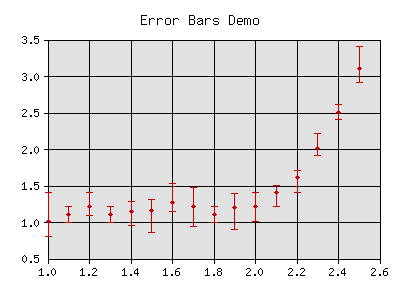
\includegraphics[scale=0.7]{error.png}
	\end{center}
	\caption{Error bars chart}
	\label{fig:error}
\end{figure}

\begin{verbatim}
use Chart::ErrorBars;
$g = Chart::ErrorBars->new();

#the x values
$g->add_dataset(qw(1   1.1  1.2  1.3  1.4  1.5  1.6  1.7  1.8  1.9  2
                   2.1 2.2  2.3  2.4  2.5));
#the y values
$g->add_dataset(qw(1   1.1  1.2  1.1  1.14 1.15 1.26 1.2  1.1  1.19 1.2
                   1.4 1.6  2.0  2.5  3.1));
#the up errors
$g->add_dataset(qw(0.4 0.1  0.2  0.1  0.14 0.15 0.26 0.27 0.1  0.19 0.2
                   0.1 0.1  0.2  0.1  0.3));
#the down errors
$g->add_dataset(qw(0.2 0.11 0.12 0.11 0.2  0.3  0.12 0.27 0.11 0.3  0.2
                   0.2 0.2  0.1  0.1  0.2));
                   
$g->set( 'xy_plot' => 'true',
         'precision' => 1,
         'pt_size' =>10, 'brush_size' => 2,
         'legend' => 'none',
         'title' => 'Error Bars Demo',
         'grid_lines' => 'true');

$g->png("errorbars.png");
\end{verbatim}

\begin{Constructor}
An instance of a error bars chart object can be created with the constructor new():
\begin{quote}
\parindent 0pt
\fett{\$obj = Chart::ErrorBars->new();}\\
\fett{\$obj = Chart::ErrorBars->new(\parameter{width}, \parameter{height});}
\end{quote}

If \textit{new()} has no arguments, the constructor returns an image with the size 300x400 pixels. If \textit{new()} has two arguments \parameter{width} and \parameter{height}, 
it returns an image with the desired size.
\end{Constructor}


\Methods
\method{All universal valid methods, see page \pageref{methods}: \class{Chart::Base}.} \\[\parabstand]


\Attributes
All universally valid options, see page \pageref{options}. Also available these special options:
\begin{description}
\item['same\_error'] Tells chart that you want to use the same error value of a data point 
     if set to true. 
     Then you have to add just one set of error values. Defaults to 'false'.
     
\item['y\_axes'] Tells chart where to place the y-axis. 
     Valid values are 'left', 'right' and 'both'. Defaults to 'left'.

\item['pt\_size']Sets the radius of the points in pixels. Default is 18.

\item['brush\_size']Sets the width of the lines in pixels. Default is 6.

\item['xy\_plot']Forces Chart to plot a x-y-graph, 
      which means that the x-axis is also numeric if set to 'true'. 
      Very useful for plots of mathematical functions. Defaults to 'false'.

\item['sort']Sorts the data of a x-y-graph ascending if set to 'true'. 
      Should be set if the added data isn't sorted. Defaults to 'false'. 
\end{description}
